\documentclass{article}


\usepackage{arxiv}

\usepackage[utf8]{inputenc} % allow utf-8 input
\usepackage[T1]{fontenc}    % use 8-bit T1 fonts
\usepackage{hyperref}       % hyperlinks
\usepackage{url}            % simple URL typesetting
\usepackage{booktabs}       % professional-quality tables
\usepackage{amsfonts}       % blackboard math symbols
\usepackage{nicefrac}       % compact symbols for 1/2, etc.
\usepackage{microtype}      % microtypography
\usepackage{lipsum}

\usepackage{graphicx}

\title{Paper title}


\author{
  Juliana Y.~Rhee\thanks{Use footnote for providing further
    information about author (webpage, alternative
    address)---\emph{not} for acknowledging funding agencies.} \\
  Center for Brain Science\\
  Department of Molecular and Cellular Biology\\
  Harvard University\\
  Cambridge, MA 02138 \\
  \texttt{rhee@g.harvard.edu} \\
  %% examples of more authors
   \And
 David D.~Cox \\
 Center for Brain Science\\
  Department of Molecular and Cellular Biology\\
  Harvard University\\
  Cambridge, MA 02138 \\
  \texttt{rhee@g.harvard.edu} \\
  %% \AND
  %% Coauthor \\
  %% Affiliation \\
  %% Address \\
  %% \texttt{email} \\
  %% \And
  %% Coauthor \\
  %% Affiliation \\
  %% Address \\
  %% \texttt{email} \\
  %% \And
  %% Coauthor \\
  %% Affiliation \\
  %% Address \\
  %% \texttt{email} \\
}

\begin{document}
\graphicspath{./figures/}

\maketitle

\begin{abstract}
%%\lipsum[1]
Text text text
\end{abstract}


% keywords can be removed
\keywords{First keyword \and Second keyword \and More}


\section{Introduction}
The brain's visual system translates ambiguous and rapidly-changing patterns of light falling on the retina into a coherent representation of the external world that can be used to guide behavior. The hierarchical organization of sensory cortex is thought to play a key role in its ability to extract and learn about latent structure from visual inputs. For example, visual object recognition in primates is thought to emerge through sequential processing across cortical areas in the ventral visual pathway~\cite{rustselectivity2010, DiCarlo:2007aa, dicarlo2012does, Chen2014682}, and numerous studies show increasing selectivity for complex stimuli at progressively higher levels of a sensory processing hierarchy~\cite{desimone1984stimulus, logothetis1996visual}. 

Similarly, learning produces distinct changes across the visual cortical hierarchy in a stimulus-specific and task-dependent way. For example, neural responses to task stimuli are specifically enhanced in inferotemporal cortex (IT), the highest level of the ventral path, after monkeys learn to discriminate complex shapes~\cite{kobatake1998shape, sigalavisual2002}. Other studies show changes in lower level areas, such as V1 or V4~\cite{schoupspractising2001, raiguellearning2006, ghose2002physiological, vogelsdoes1994} when simpler stimuli are used, as in orientation discrimination tasks. In all cases, perceptual learning results in specific changes in neural representations~\cite{goldstone1998perceptual, fine2002comparing, OpdeBeeck201022}. However, the nature of the transformations that occur from one level of the hierarchy to the next remain poorly understood. 


\section{Retinotopic organization of rat visual cortex}
\label{sec:headings}

Text goes here.

\subsection{Headings: second level}
\lipsum[5]

\begin{figure}[ht]
  \centering
  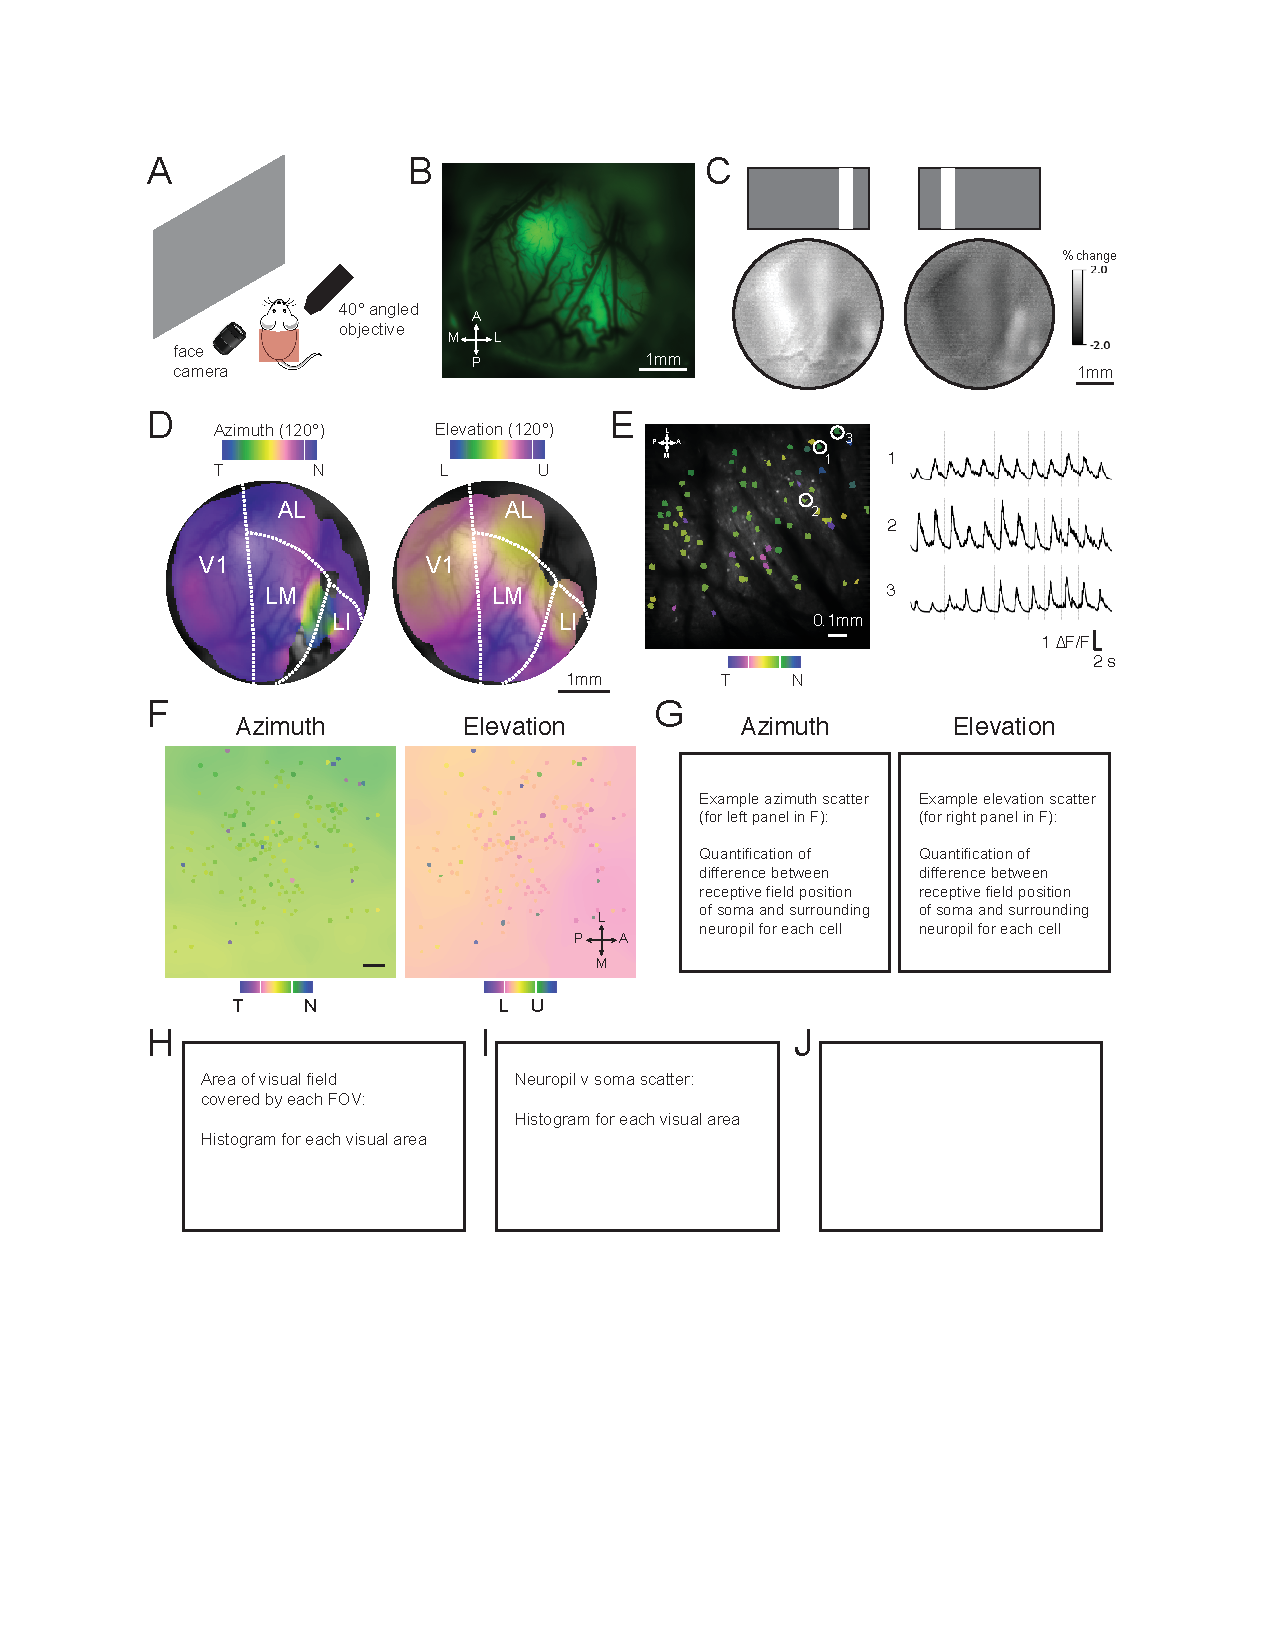
\includegraphics{figures/retino.pdf}
  \caption{Sample figure caption.}
  \label{fig:fig1}
\end{figure}

\subsubsection{Headings: third level}
\lipsum[6]


\section{Examples of citations, figures, tables, references}
\label{sec:others}
\lipsum[8] \cite{kour2014real,kour2014fast} and see \cite{hadash2018estimate}.

The documentation for \verb+natbib+ may be found at
\begin{center}
  \url{http://mirrors.ctan.org/macros/latex/contrib/natbib/natnotes.pdf}
\end{center}
Of note is the command \verb+\citet+, which produces citations
appropriate for use in inline text.  For example,
\begin{verbatim}
   \citet{hasselmo} investigated\dots
\end{verbatim}
produces
\begin{quote}
  Hasselmo, et al.\ (1995) investigated\dots
\end{quote}

\begin{center}
  \url{https://www.ctan.org/pkg/booktabs}
\end{center}


\subsection{Figures}
\lipsum[10] 
See Figure \ref{fig:fig1}. Here is how you add footnotes. \footnote{Sample of the first footnote.}
\lipsum[11] 

\begin{figure}
  \centering
  \fbox{\rule[-.5cm]{4cm}{4cm} \rule[-.5cm]{4cm}{0cm}}
  \caption{Sample figure caption.}
  \label{fig:fig1}
\end{figure}

\subsection{Tables}
\lipsum[12]
See awesome Table~\ref{tab:table}.

\begin{table}
 \caption{Sample table title}
  \centering
  \begin{tabular}{lll}
    \toprule
    \multicolumn{2}{c}{Part}                   \\
    \cmidrule(r){1-2}
    Name     & Description     & Size ($\mu$m) \\
    \midrule
    Dendrite & Input terminal  & $\sim$100     \\
    Axon     & Output terminal & $\sim$10      \\
    Soma     & Cell body       & up to $10^6$  \\
    \bottomrule
  \end{tabular}
  \label{tab:table}
\end{table}

\subsection{Lists}
\begin{itemize}
\item Lorem ipsum dolor sit amet
\item consectetur adipiscing elit. 
\item Aliquam dignissim blandit est, in dictum tortor gravida eget. In ac rutrum magna.
\end{itemize}


\bibliographystyle{unsrt}  
%\bibliography{references}  %%% Remove comment to use the external .bib file (using bibtex).
%%% and comment out the ``thebibliography'' section.


%%% Comment out this section when you \bibliography{references} is enabled.
\begin{thebibliography}{1}

\bibitem{kour2014real}
George Kour and Raid Saabne.
\newblock Real-time segmentation of on-line handwritten arabic script.
\newblock In {\em Frontiers in Handwriting Recognition (ICFHR), 2014 14th
  International Conference on}, pages 417--422. IEEE, 2014.

\bibitem{kour2014fast}
George Kour and Raid Saabne.
\newblock Fast classification of handwritten on-line arabic characters.
\newblock In {\em Soft Computing and Pattern Recognition (SoCPaR), 2014 6th
  International Conference of}, pages 312--318. IEEE, 2014.

\bibitem{hadash2018estimate}
Guy Hadash, Einat Kermany, Boaz Carmeli, Ofer Lavi, George Kour, and Alon
  Jacovi.
\newblock Estimate and replace: A novel approach to integrating deep neural
  networks with existing applications.
\newblock {\em arXiv preprint arXiv:1804.09028}, 2018.

\end{thebibliography}


\end{document}
